In this section, the layer is described in some detail in terms of its specific subsystems. Describe each of the layers and its subsystems in a separate chapter/major subsection of this document. The content of each subsystem description should be similar. Include in this section any special considerations and/or trade-offs considered for the approach you have chosen.

\subsection{Audio Amplifier}
This section should be a general description of a particular subsystem for the given layer. For most subsystems, an extract of the architectural block diagram with data flows is useful. This should consist of the subsystem being described and those subsystems with which it communicates.

\begin{figure}[h!]
	\centering
 	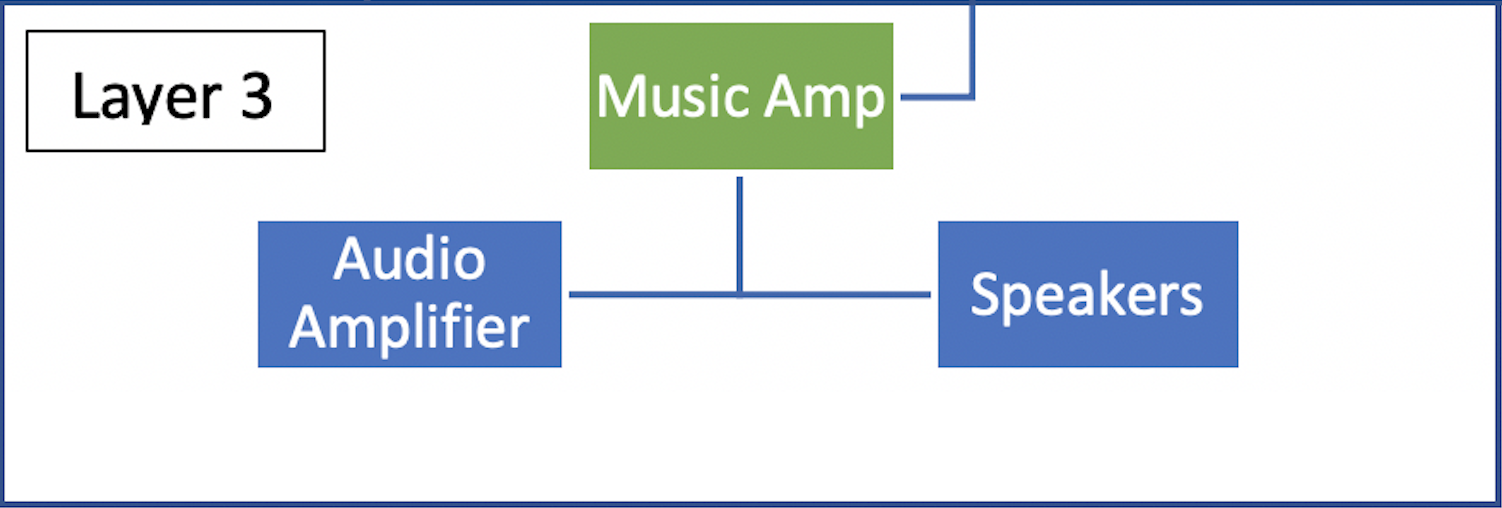
\includegraphics[width=0.60\textwidth]{images/subsystem3}
 \caption{Example subsystem description diagram}
\end{figure}

\subsubsection{Assumptions}
Any assumptions made in the definition of the subsystem should be listed and described. Pay particular attention to assumptions concerning interfaces and interactions with other layers.

\subsubsection{Responsibilities}
Each of the responsibilities/features/functions/services of the subsystem as identified in the architectural summary must be expanded to more detailed responsibilities. These responsibilities form the basis for the identification of the finer-grained responsibilities of the layer's internal subsystems. Clearly describe what each subsystem does.

\subsubsection{Subsystem Interfaces}
Each of the inputs and outputs for the subsystem are defined here. Create a table with an entry for each labelled interface that connects to this subsystem. For each entry, describe any incoming and outgoing data elements will pass through this interface.

\begin {table}[H]
\caption {Subsystem interfaces} 
\begin{center}
    \begin{tabular}{ | p{1cm} | p{6cm} | p{3cm} | p{3cm} |}
    \hline
    ID & Description & Inputs & Outputs \\ \hline
    \#xx & Description of the interface/bus & \pbox{3cm}{input 1 \\ input 2} & \pbox{3cm}{output 1}  \\ \hline
    \#xx & Description of the interface/bus & \pbox{3cm}{N/A} & \pbox{3cm}{output 1}  \\ \hline
    \end{tabular}
\end{center}
\end{table}

\subsection{Speakers}
The speakers are one of the last, most straightforward systems in the vest. There will be three sets of speakers for different frequencies: lows, mids, and highs. These will act as the shakers for the vest. The speakers will also act simply as a medium for output, and will do no heavy-duty signal processing of their own. It will be connected to the music amp and the audio amplifier. The speakers are a black-box system that will not be designed by the team.

\begin{figure}[h!]
	\centering
 	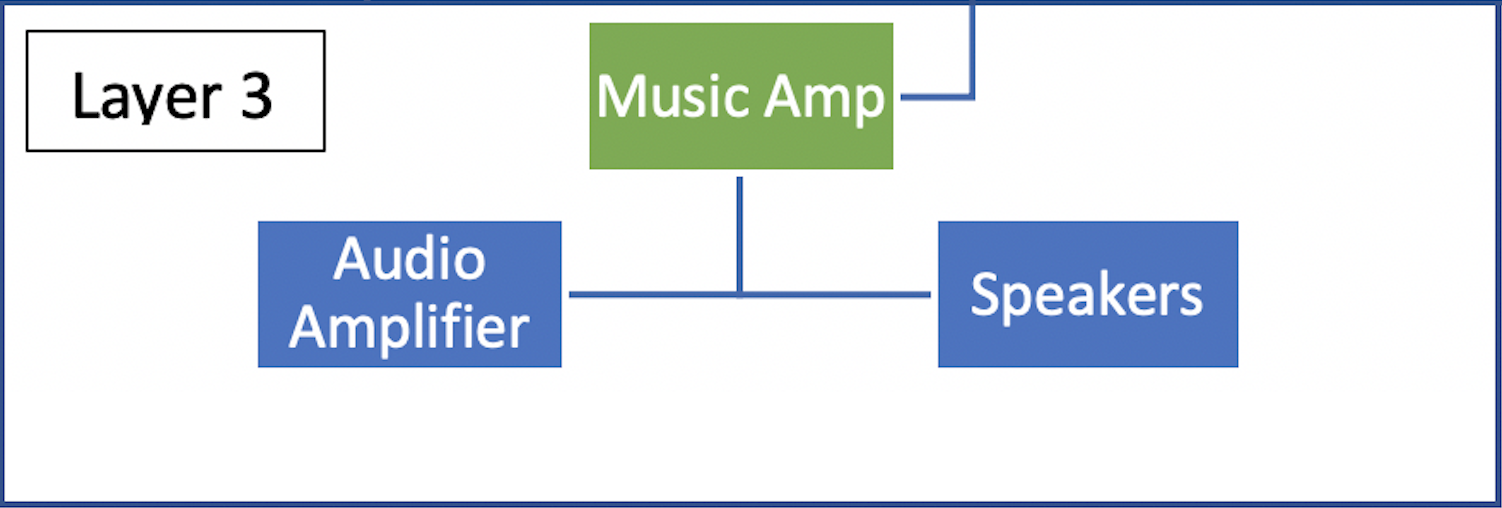
\includegraphics[width=0.60\textwidth]{images/subsystem3}
 \caption{Example subsystem description diagram}
\end{figure}

\subsubsection{Assumptions}
It is assumed that there will be speakers available that will fit our specifications and that will be able to comfortably and safely fit in the vest. We also assume that there are speakers powerful enough to emit vibrations that can be felt through the vest we will use.

\subsubsection{Responsibilities}
The speakers have few responsibilities, in terms of custom functionality. They are simply meant to be the medium through which the user will feel the music/vibrations.

\subsubsection{Subsystem Interfaces}

\begin {table}[H]
\caption {Subsystem interfaces} 
\begin{center}
    \begin{tabular}{ | p{1cm} | p{6cm} | p{3cm} | p{3cm} |}
    \hline
    ID & Description & Inputs & Outputs \\ \hline
    \#1 & Connection to audio amplifier & \pbox{3cm}{ Audio amplification settings } & \pbox{3cm}{ Change in audio/vibration characteristics in vest }  \\ \hline
    \#2 & Connection to music amplifier & \pbox{3cm}{ NA } & \pbox{3cm}{ Speakers receive amplified audio/music signals ready for output }  \\ \hline
    \end{tabular}
\end{center}
\end{table}

